\section{Loops}

Looping is a fundamental concept in computer programming. Loops allow for repetition of actions or tasks. As we stated in the previous section on recursion, any tail recursive algorithm may be translated into an algorithm that uses loops. In this section, we will describe this translation pipeline as a sequence of steps, then begin to distance ourselves from recursion when it is suboptimal.

\subsection{Translation Pipeline for Tail Recursive Methods}
\subsubsection*{A Coarse-Grained Approach}
What follows is a high-level introduction to converting from tail recursive methods to iteration. While you may not understand everything at first, we supplement this with a comprehensive translation schema.

Writing recursive methods is certainly fun.\footnote{The definition of ``fun'' is, of course, relative.} Though, the use of recursion is not always the most intuitive approach to solve a problem according to some programmers/students. Many programming languages offer emph{iteration} statements, which allow us to perform a task that we might otherwise use recursion to complete. Suppose we have a standard recursive emph{fact} method. 
\begin{clrr}[]{Standard Recursive Factorial}
\begin{lstlisting}[language=MyJava]
static int fact(int n) {
  if (isZero(n)) { 
    return 1; 
  } else {
    return n * fact(n - 1);
  }
}
\end{lstlisting}
\tcblower
\begin{lstlisting}[language=MyJavaNLN]
static int factTR(int n, int acc) {
  if (isZero(n)) { 
    return acc; 
  } else {
    return factTR(subOne(n), n * acc);
  }
}
\end{lstlisting}
\end{clrr}
The first step in converting a recursive method into its iterative counterpart is to rewrite it using tail recursion. Something we, of course, already know how to do from the previous section. 
Notice that, in order to ``tail-recursify'' \texttt{fact}, we had to add an extra parameter that keeps track of the ``current result.''\footnote{Some tail recursive methods need more than one extra parameter---it is a case-by-case basis.} The reason for converting recursive methods into tail recursion is because of their direct relation to iteration.\footnote{A method definition may already be tail recursive depending on the circumstance.} Let us look a little deeper into this and find out why.

Our iterative version of \texttt{fact} should move all ``accumulator'' variables into the method body. E.g., \texttt{acc} will now be declared locally to the \texttt{fact} method. In addition to this movement, all accumulator-to-local variables should have an ``iterative purpose statement,'' which mimics the documentation comment for the accumulator parameter.

\begin{cl}[]{Localizing Accumulator Variables}
\begin{lstlisting}[language=MyJava]
static int fact(int n) {
  // acc stores the current factorial value as n goes to zero.
  int acc = 1;
  // TODO.
}
\end{lstlisting}
\end{cl}

Second, we must describe the syntax of a loop. A \texttt{while} loop is the construct of choice, and it has two components: a condition denoted as a predicate, and a body. The loop checks to see if the given predicate is true and, if so, executes the body of the loop. On the other hand, if the predicate is false, we jump down to below the loop. Each pass through the loop, it re-verifies that the predicate holds true. Unlike expressions, however, a \texttt{while} loop, itself, does not resolve to some value. It is called a emph{statement} because of this property. Let us begin by defining the predicate of our loop. To answer this, we ask, then answer, the question of the base case(s) for our tail recursive method. As we see, our base case is true when $n$ is zero. Therefore our loop should continue to execute as long as $n$ is not zero. One tail recursive method call correlates directly with one loop iteration. So, let us remove the \texttt{if}/\texttt{else} statement chain and substitute them by a loop whose condition is nothing more than the negated base case(s).

\begin{cl}[]{Adding the Loop and Negated Predicate}
\begin{lstlisting}[language=MyJava]
static int fact(n) {
  // acc stores the current factorial value as n goes to zero.
  int acc = 1;
  while (!(n == 0)) {
    // TODO.
  }
}
\end{lstlisting}
\end{cl}

Finally, we come to the heart of the loop. Within, we update variables according to how they are updated in the tail recursive call. Namely, as we saw, $n$ is decremented by $1$, and $emph{acc}$ is multiplied by $n$. We must be careful, however, because the order of these statements is significant! In the tail recursive method call to \texttt{fact}, the $n$ that is decremented is passed to the method, whereas the original value of $n$ is used when multiplying by $emph{acc}$. As a result, the accumulator update should come first.

\begin{cl}[]{Loop Body Becomes Tail Recursive Updates}
\begin{lstlisting}[language=MyJava]
static int fact(int n) {
  // acc stores the current factorial value as n goes to zero.
  int acc = 1;
  while (!(n == 0)) {
    acc = acc * n;
    n = n - 1;
  }
}
\end{lstlisting}
\end{cl}

We are almost done. The loop body is now complete, with each modification pairing precisely with some piece of the tail recursive version. All that remains is the base case return statement. In our tail recursive method, once we hit the base case, we return \texttt{acc}. We model this, of course, using a return outside the loop.

\begin{cl}[]{Return the Base Case}
\begin{lstlisting}[language=MyJava]
static int fact(int n) {
  // acc stores the current factorial value as n goes to zero.
  int acc = 1;
  while (!(n == 0)) {
    acc = acc * n;
    n = n - 1;
  }
  return acc;
}
\end{lstlisting}
\end{cl}

Excellent, we now have an iterative version of the factorial method! Let us compare these two side-by-side, color-coding their similarities. Base cases are \textcolor{red}{red}, accumulated variables/steps are \textcolor{darkyellow}{yellow}, and return values are \textcolor{darkgreen}{green}. 

\begin{clrr}[]{Tail Recursive versus Iterative Factorial}
\begin{lstlisting}[language=MyJava]
static int fact(int n, int acc) {
  if (*;\textcolor{red}{(n == 0)};*) {
    return (*;\textcolor{darkgreen}{acc};*);
  } else {
    return fact((*;\textcolor{darkyellow}{n - 1};*), (*;\textcolor{darkyellow}{acc * n};*));
  }
}
(*;\phantom{};*)
(*;\phantom{};*)
(*;\phantom{};*)
\end{lstlisting}
\tcblower
\begin{lstlisting}[language=MyJavaNLN]
static int fact(int n) {
  // acc stores the current factorial
  // value as n goes to zero.
  int acc = 1;
  while (!(*;\textcolor{red}{(n == 0)};*)) {
    (*;\textcolor{darkyellow}{acc = acc * n};*);
    (*;\textcolor{darkyellow}{n = n - 1};*);
  }
  return (*;\textcolor{darkgreen}{acc};*);
}
\end{lstlisting}
\end{clrr}

\subsubsection*{A Fine-Grained Approach}
What we just saw was a fast-paced, high-level overview of the conversion process from tail recursive methods into methods that use while loops. Let’s take a step back and slow our approach to better understand each piece. We first want to describe a general outline of the steps to success in this translation pipeline. 

Of course, the goal, in due time, is to work our way from $TR$ to $I$, but there are a few highly important intermediary components to this process. Note that the lines from $P$ to $R$, and $R$ to $TR$ are not as important for this section of the transformation.

\begin{figure}[h!]
\centering
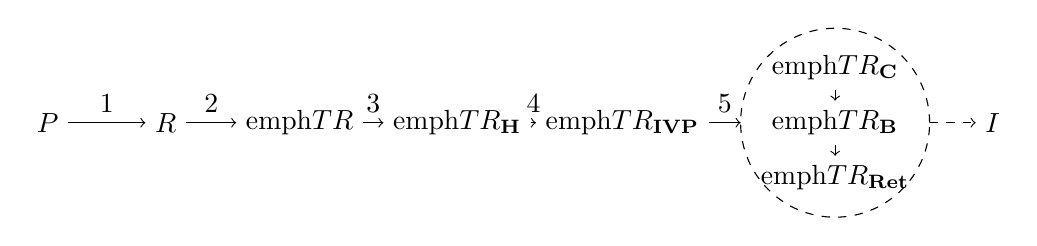
\begin{tikzpicture}
  % Define nodes for all elements
  \node (P) at (-2,0) {$P$};
  \node (R) at (-0.5,0) {$R$};
  \node (TR) at (1.2,0) {emph{$TR$}};
  \node (TRH) at (3.2,0) {emph{$TR_\mathbf{H}$}};
  \node (TRIVP) at (5.3,0) {emph{$TR_\mathbf{IVP}$}};
  \node (TRC) at (8,0.7) {emph{$TR_\mathbf{C}$}};
  \node (TRB) at (8,0) {emph{$TR_\mathbf{B}$}};
  \node (TRRet) at (8,-0.7) {emph{$TR_\mathbf{Ret}$}};
  \node (I) at (10,0) {$I$};

  % Draw arrows
  \draw[->] (P) -- (R) node[midway, above] {1};
  \draw[->] (R) -- (TR) node[midway, above] {2};
  \draw[->] (TR) -- (TRH) node[midway, above] {3};
  \draw[->] (TRH) -- (TRIVP) node[midway, above] {4};
  \draw[->] (TRIVP) -- (6.8,0) node[midway, above] {5};
  \draw[->] (TRC) -- (TRB);
  \draw[->] (TRB) -- (TRRet);
  
  % Draw dashed circle
  \draw[dashed] (8,0) circle (1.2);
  \draw[dashed,->] (9.2,0) -- (I);

\end{tikzpicture}
\caption{Fine-Grained Translation Pipeline}
\end{figure}

$TR$ is the tail recursive method derived either from the problem statement $P$ or the standard recursive step $R$. From here, we make our way to emph{$TR_\mathbf{H}$}, denoting the ``color-coding'' phase, where we mark the three sub components of a tail recursive method, those being the base case(s), updated variables in the tail recursive call, and returned values from the base case. 

emph{$TR_\mathbf{IVP}$}, or ``Iterative Variable Purpose,'' is a step following the method signature, but preceding the loop definition. In this step, we examine the updated variables/accumulators marked in emph{$TR_\mathbf{H}$} and localize them into variables not passed as arguments to a method, but rather as a sequence of value updates. Moreover, we add comments to these variable declarations explaining their purpose.

emph{$TR_\mathbf{C}$} is the step wherein we write the \ttt{while} keyword, followed by the negated base case condition(s) as a series of conjunctions.

emph{$TR_\mathbf{B}$} is where we design the body of our loop, which contains update statements to our localized iterative variables rather than arguments to a recursive call.

Finally, in emph{$TR_\mathbf{Ret}$}, we add the line to return the accumulated local variable(s). $I$ is the output translation.

\subsection{emph{$TR_\mathbf{H}$:}} When designing a tail recursive method, there are several values to keep in mind: base cases (i.e., terminating conditions), returned values that are not method calls, and accumulators. Each of these play a crucial role in the transition to $I$, and quickly yet correctly identifying these as they fit in tail recursive methods is paramount. Let us re-look at our old factorial friend to see what this entails.

\begin{cl}[]{Tail Recursive Factorial}
\begin{lstlisting}[language=MyJava]
static int fact(int n, int acc) {
  if (n == 0) {
    return acc;
  } else {
    return fact(n - 1, acc * n);
  }
}
\end{lstlisting}
\end{cl}

Marking the base case(s) is usually rather simple, as they are most often the selection statements that return a value rather than a recursive method invocation. So, the only instance of this in the above definition is $n == 0$. So, we highlight this in a color, e.g., \textcolor{red}{red}.

\begin{cl}[]{Highlighting Factorial Base Case}
\begin{lstlisting}[language=MyJava]
static int fact(int n, int acc) {
  if ((*;\textcolor{red}{n == 0};*)) {
    return acc;
  } else {
    return fact(n - 1, acc * n);
  }
}
\end{lstlisting}
\end{cl}

To coincide with the base case(s), we also want to highlight the returned values that are not recursive calls. Only one exists, namely $emph{acc}$. Let us highlight this in \textcolor{darkgreen}{green}.

\begin{cl}[]{Highlighting Factorial Returned Values}
\begin{lstlisting}[language=MyJava]
static int fact(int n, int acc) {
  if ((*;\textcolor{red}{n == 0};*)) {
    return (*;\textcolor{darkgreen}{acc};*);
  } else {
    return fact(n - 1, acc * n);
  }
}
\end{lstlisting}
\end{cl}

We are almost done. Now, we want to highlight variables passed to the (tail) recursive call that are updated. When we say updated, we mean ``modified'' insofar as they are not simply copied verbatim, e.g., $f(n) = f(n)$, in which we see $n$ remains unaltered. Fortunately, both $n$ and $emph{acc}$ are updated ($n$ is decremented by one; $emph{acc}$ is multiplied by $n$). Let us highlight these changes in \textcolor{darkyellow}{yellow}. 

\begin{cl}[]{Highlighting Factorial Updated Arguments}
\begin{lstlisting}[language=MyJava]
static int fact(int n, int acc) {
  if ((*;\textcolor{red}{n == 0};*)) {
    return (*;\textcolor{darkgreen}{acc};*);
  } else {
    return fact((*;\textcolor{darkyellow}{n - 1};*), (*;\textcolor{darkyellow}{acc * n};*));
  }
}
\end{lstlisting}
\end{cl}

\subsection{emph{$TR_\mathbf{IVP}$}:} All accumulator variables in tail recursive methods serve some purpose, one way or another, hence their necessity. The same holds true for local variables defined to substitute accumulators. Conveniently enough, every variable designated as an accumulator morphs nicely into a local variable when writing the iterative counterpart. Consider, once more, the tail recursive factorial definition. We use $emph{acc}$ to accumulate the result as a parameter, indicating the need for an accumulator statement. We can simply insert this as an addendum to our Java documentation comment.

\begin{cl}[]{Accumulator Statement for Factorial}
\begin{lstlisting}[language=MyJava]
/**
 * @accumulator acc stores the current factorial product. 
 */
static int fact(int n, int acc) {
  if ((*;\textcolor{red}{n == 0};*)) {
    return (*;\textcolor{darkgreen}{acc};*);
  } else {
    return fact((*;\textcolor{darkyellow}{n - 1};*), (*;\textcolor{darkyellow}{acc * n};*));
  }
}
\end{lstlisting}
\end{cl}

In the translation to a loop, we move $emph{acc}$ to the body of the method, and write a similar iterative variable purpose.\footnote{By ``move,'' we mean ``remove'' but not ``delete.''} Note that the value the initialized variable receives depends on the problem/context, but it always matches whatever value is passed to a tail recursive helper method.

\begin{cl}[]{Iterative Variable Purpose Statement}
\begin{lstlisting}[language=MyJava]
static int fact(int n) {
  // acc stores the current factorial product. 
  int acc = 1;
}
\end{lstlisting}
\end{cl}

Writing these imperative variable purposes, akin to accumulator statements, helps us organize what variables change and, more importantly, when and how they change. 

\subsection{emph{$TR_\mathbf{C}$}:} Up next is where we take our base case condition, highlighted in red, and insert it as the negated condition for our loop. First, we add the \ttt{while} keyword to our method, then follow this with a set of parentheses and an exclamation point immediately after the opening parenthesis but before the closing. Inside these parentheses we insert the base case condition. To be safe, you should also insert parentheses for the base case, which ensures that the correct expression is negated by the logical `not' operator. Follow this with an opening and closing brace set.

\begin{cl}[]{Adding Condition to Loop}
\begin{lstlisting}[language=MyJava]
static int fact(int n) {
  // acc stores the current factorial product. 
  int acc = 1;
  while (!(n == 0)) { 
    // TODO.
  }
}
\end{lstlisting}
\end{cl}

\subsection{emph{$TR_\mathbf{B}$}:} Finally we get to the fun part of this translation process: the body of our loop. Here we need to make a design choice of what variables to update and when they should be updated. We take the \textcolor{darkyellow}{yellow} highlighted tail recursive arguments, create assignment statements out of them, and insert them into the body of our loop. To do so, we need to follow two principles:

\textbf{Rule of Reassignment}: In any tail recursive call, if we pass an expression $e$ which updates parameter $p$, then in the loop body, we directly reassign $p$ to $e$.

\textbf{Rule of Update}: If we have two parameters $p$ and $q$ that are updated as part of the tail recursive call, and $p$'s value is used as part of updating $q$, then $q$ must be modified before $p$.

The rule of reassignment is straightforward: we have an expression that resolves to some value, which corresponds precisely to those highlighted arguments. This expression is converted into an assignment statement to the locally-declared variable. 

The rule of update, on the other hand, is not as straightforward. Essentially, we use this rule to ensure that variables whose value depends on another are not prematurely updated. Consider the following incorrect update of $n$ before updating $emph{acc}$:
\begin{figure}[H]
\centering
\begin{minipage}{.4\textwidth}
  \begin{align*}
  &\texttt{n = n - 1}\\
  &\texttt{acc = acc * n}
  \end{align*}
\end{minipage}%
\begin{minipage}{.4\textwidth}
\begin{tabular}{c|c|c}
Iteration \# & \texttt{n} & \texttt{acc}\\
\hline
\hline
0 & 5 & 1\\
\hline
1 & 4 & 4\\
\hline
2 & 3 & 12\\
\hline
3 & 2 & 24\\
\hline
4 & 1 & 24\\
\hline
5 & 0 & 0\\
\end{tabular}
\end{minipage}
\end{figure}
We see that this variable update ordering produces $0$, which does not match our recursive trace! We get zero thanks in part due to the final multiplication before our loop condition is falsified. Let us now try the other possible ordering, in which $emph{acc}$ is updated before $n$. Hence, we are now in the second attempt of completing $TR_emph{B}$:
\begin{figure}[H]
\centering
\begin{minipage}{.4\textwidth}
  \begin{align*}
  &\texttt{acc = acc * n}\\
  &\texttt{n = n - 1}
  \end{align*}
\end{minipage}%
\begin{minipage}{.4\textwidth}
\begin{tabular}{c|c|c}
Iteration \# & \texttt{n} & \texttt{acc}\\
\hline
\hline
0 & 5 & 1\\
\hline
1 & 4 & 5\\
\hline
2 & 3 & 20\\
\hline
3 & 2 & 60\\
\hline
4 & 1 & 120\\
\hline
5 & 0 & 120\\
\end{tabular}
\end{minipage}
\end{figure}
This results in $120$, which matches our recursive trace. Therefore, without loss of generality, we can conclude that we should update the accumulator variable before updating $n$ in this circumstance.

Determining the correct order of update, according to the rules we specify, may take a few tries to get right. The idea is to match the result of a tail recursive trace done previously that is known to be correct.

\subsection{emph{$TR_\mathbf{Ret}$}:}
In our final stage of translation, we add the necessary return statement(s) that serve to return the accumulated result from our loop. We highlighted these values in \textcolor{darkgreen}{green} during the highlighting/color-coding stage.
\begin{cl}[]{Adding Accumulator Return Statement to Loop}
\begin{lstlisting}[language=MyJava]
static int fact(int n) {
  // acc stores the current factorial product. 
  int acc = 1;
  while (!(n == 0)) { 
    acc = acc * n;
    n = n - 1;
  }
  return acc;
}
\end{lstlisting}
\end{cl}

And that is it; the translation pipeline is complete, and we now know how to translate a tail recursive method into one that uses a loop.

The astute reader might question the need for a tail recursion-to-iteration translation schema. We mentioned the term tail call optimization in the previous section on recursion, and will now explain the relation to loops.

Recall the benefit of tail recursion over standard recursion: it uses only one (replaceable) activation record. Though, because we can translate any tail recursive method into an iterative algorithm, we forgo the stack in its entirety.

From here we might ask a similar question: can we translate any standard recursive method into one that uses tail recursion (and by transitivity, iteration)? In general, the answer is yes, through a concept called emph{continuation-passing style}\index{continuation-passing style}. Because of how difficult it is to implement continuations in Java, we will omit any further discussion, but interested readers should delve into functional programming if this equivalence is intriguing.

\section{Iteration Constructs}

Perhaps the related equivalence to tail recursion is too abstract for some to digest. Indeed, we believe the relationship is somewhat far-fetched at first glance, but after enough practice, it becomes clear. We will now discuss loops from a non-translation perspective. That is, if we assume the translation diagram from before, we are going straight from the problem statement $P$ to the iterative solution $I$.

As we stated, loops are statements in Java, meaning they do not, themselves, resolve to a value. Therefore any and all lines of code executed inside the body of a loop must be statements rather than expressions.

\example{Suppose we want to print the first one hundred prime integers. Recall the definition of primality: a positive integer $n$ is prime if it is divisible by only one and itself. Without loops, we would otherwise solve this task using recursion. Although summing prime values is not a too terribly complicated task, it requires a bit of a verbose set of methods, should we choose to do it tail recursively. Instead, let us try and use loops to our advantage. We want to continue looping until we have summed one hundred prime values. Fortunately there is exactly one correct test case for this method, so writing an elaborate test suite is superfluous.}

Declaring an integer counter $c$ is mandatory. Our loop condition, therefore, is to continue so long as we have not reached one hundred prime values. When designing loop conditions, we ask ourselves the question, ``What should be true after the loop?,'' and design the condition around the answer. Our counter $c$ will be exactly one hundred upon loop completion, so the condition is the negated version of this expression.\footnote{Rather than \ttt{(!(c == 100))}, we can write \ttt{(c != 100)} to achieve the same effect.}

Up next we need a method to determine if a value is prime. We presented the definition of primality before, and it is also known that we only need to check up to the square root of $n$ for primality. Let us design such a method, writing the appropriate tests. Our condition is to continue so long as a variable, $i$, is less than or equal to the square root of our input number. The variable $i$ serves as a counter towards our number; if we find that $n$ is not divisible by any numbers from two up to the square root of $n$, then it must be prime.\footnote{We cast the result of \ttt{Math.sqrt} to an integer because it returns a \ttt{double} rather than an \ttt{int} datatype.} Note the edge cases of zero and one, which are both non-prime.

\begin{cl}[SumPrimes.java]{Sum Of First 100 Primes Skeleton}
\begin{lstlisting}[language=MyJava]
class SumPrimes {

  /**
   * Computes the sum of the first 100 prime integers.
   * @return sum of first 100 primes.
   */
  static int sum100Primes() {
    int c = 0;
    while (c != 100) { /* TODO. */ }
    return 0;
  }
}
\end{lstlisting}
\end{cl}

\begin{cl}[PrimeTester.java]{Loop Primality Tests}
\begin{lstlisting}[language=MyJava]
import static Assertions.assertAll;
import static Assertions.assertTrue;
import static Assertions.assertFalse;
import static Prime.isPrime;

class PrimeTester {

  @Test
  void testPrime() {
    assertAll(
      () -> assertTrue(isPrime(17)),
      () -> assertTrue(isPrime(101)),
      () -> assertTrue(isPrime(3)),
      () -> assertTrue(isPrime(9173)),
      () -> assertFalse(isPrime(0)),
      () -> assertFalse(isPrime(1)),
      () -> assertFalse(isPrime(2)),
      () -> assertFalse(isPrime(202)),
      () -> assertFalse(isPrime(213123447)));
  }
}
\end{lstlisting}
\end{cl}

\begin{cl}[Prime.java]{Loop Primality Implementation}
\begin{lstlisting}[language=MyJava]
class Prime {

  /**
   * Determines if a given integer is prime.
   * 
   * @param n positive integer.
   * @return true if prime, false otherwise.
   */
  static boolean isPrime(int n) {
    if (n < 2) { 
      return false;
    } else {
      int bound = (int) Math.sqrt(n);
      int i = 2;
      while (i <= bound) {
        if (n % i == 0) {
          return false;
        }
        i++;
      }
      return true;
    }
  }
}
\end{lstlisting}
\end{cl}

The primality tests pass, which means we can put \ttt{isPrime} to work inside of \ttt{sum100Primes}. The method logic is straightforward: initialize our counter c at one. We also need a variable to track the last-found prime integer, so we know from where to start the search. We will call this variable $l$ and initialize it to zero. Finally, a $\mathit{sum}$ variable accumulates the sum of each prime. Inside the loop, we declare another variable $v$, which serves as the value to check for primality, taking on the value of $l + 1$ (if it were just $l$, we would forever check the same value for primality!). Run $v$ through the \ttt{isPrime} method and, if it is prime, assign to $l$ the value of $v$, add $v$ to the sum, and increment $c$. Otherwise, increment $l$ by one.\footnote{We will note that this code is overly verbose for pedagogical purposes.}

\begin{cl}[SumPrimes.java]{Sum Of First 100 Primes Implementation}
\begin{lstlisting}[language=MyJava]
class SumPrimes {

  /**
   * Computes the sum of the first 100 prime integers.
   * @return sum of first 100 primes.
   */
  static int sum100Primes() {
    // Counter for no. of primes.
    int c = 0;   
    // Current "prime value".
    int l = 0;   
    // Running sum.
    int sum = 0; 
    
    while (c != 100) {
      int v = l + 1;
      if (isPrime(v)) {
        l = v;
        sum += v;
        c++;
      } else {
        l++;
      }
    }
    return sum;
  }
}
\end{lstlisting}
\end{cl}

Running the code produces $24133$: the desired answer.

\example{Suppose we want to compute the sum of the first $n$ odd reciprocals. That is, $\frac{1}{1} + \frac{1}{3} + \frac{1}{5} + \cdots + \frac{1}{2n-1}$. Again, we might do this recursively, but let us try and write an iterative algorithm. The signature is straightforward: we want to receive some integer $n$ and compute the sum of $n$ odd reciprocals. Our tests are trivial to write with the employment of a calculator.}

\begin{cl}[OddReciprocalSumTester.java]{Odd Reciprocal Summation Tests}
\begin{lstlisting}[language=MyJava]
import static Assertions.assertAll;
import static Assertions.assertEquals;
import static OddReciprocalSum.oddRecipSum;

class OddReciprocalSumTester {

  private static final double DELTA = 0.001;

  @Test
  void testOddRecipSum() {
    assertAll(
      // 1/1 + 1/3 + 1/5 + 1/7.
      () -> assertEquals(1.67619, oddRecipSum(4), DELTA),
      // Sum of zero reciprocals is zero.
      () -> assertEquals(0, oddRecipSum(0), DELTA),
      // 1/1.
      () -> assertEquals(1, oddRecipSum(1), DELTA),
      // 1/1 + 1/3 + 1/5 + 1/7 + 1/9 + 1/13 + ...
      () -> assertEquals(2.26435, oddRecipSum(13), DELTA));
  }
}
\end{lstlisting}
\end{cl}

The implementation is similarly simple: we create a counter $c$ that increments so long as $c$ is not equal to $n$, accumulating the $emph{sum}$ of $1$ divided by $2c-1$.

\begin{cl}[OddReciprocalSum.java]{Odd Reciprocal Summation Implementation}
\begin{lstlisting}[language=MyJava]
class OddReciprocalSum {

  /**
   * Computes the sum of the first n odd reciprocals.
   * @param n number of reciprocals to compute.
   * @param sum of n odd reciprocals.
   * @return sum of first n odd reciprocals.
   */
  static double oddRecipSum(int n) {
    int c = 0;
    double sum = 0;
    while (c != n) {
      sum += c / (double) (2 * c - 1)
      c++;
    }
    return sum;
  }
}
\end{lstlisting}
\end{cl}

Note the cast of the denominator from an \ttt{int} to a \ttt{double}; what happens if we omit the cast? Our tests fail because dividing two integers produces another integer, which is not desired when all of our numbers are less than or equal to one.\footnote{Equivalently, we might multiply $c$ by $2.0$, or subtract $1.0$; all of these coerce the \ttt{int} into a \ttt{double}, thereby allowing correct division.}

While loops are reserved for when cases of termination are unknown. That is, we may or may not know when a while loop condition becomes false. Thus far, all methods that we have written use deterministic and predictable termination cases; we increment a counter until hitting some upper-bound. The use of \ttt{while} is unnecessary in these circumstances due to the equivalent \ttt{for} construct.

With a \ttt{for} loop, we provide three values: an emph{initializer statement}, a conditional expression, and a emph{step statement}. We have previously seen conditional expressions as they are the basis for our \ttt{while} condition. An initializer statement, as its name suggests, declares a variable and initializes it to some value. Stepping statements determine how to change a value between iterations of the loop. In our \ttt{while} loops, notice how we always incremented the counter by one at the end of the loop. Stepping statements take care of this for us, reducing the need for such simple statements in the loop body.

\example{Suppose we wish to write a program that returns the sum of the integers between two integers $a$ and $b$, inclusive. We know how many integers there are between $a$ and $b$, assuming $a \leq b$, so we should use a \ttt{for} loop to solve this problem.} 

\begin{cl}[SumIntervalTester.java]{Sum of Integers in the Interval $[a, b]$}
\begin{lstlisting}[language=MyJava]
import static Assertions.assertAll;
import static Assertions.assertEquals;
import static SumInterval.sum;

class SumIntervalTester {

  @Test
  void testSumInterval() {
    assertAll(
      () -> assertEquals(0, sum(5, 0)),
      () -> assertEquals(0, sum(0, 0)),
      () -> assertEquals(55, sum(0, 10)),
      () -> assertEquals(55, sum(1, 10)),
      () -> assertEquals(110, sum(5, 15)));
  }
}
\end{lstlisting}
\end{cl}

We want to iterate from $i = a$ so long as $i \leq b$. We use the variable $i$ out of convention; one could easily use any other unused identifier.

\begin{cl}[SumInterval.java]{Sum of Integers in the Interval $[a, b]$}
\begin{lstlisting}[language=MyJava]
class SumInterval {

  /**
   * Computes the sum of the integers between a and b inclusive.
   * @param a lower-bound inclusive.
   * @param b upper-bound inclusive.
   * @return sum of values.
   */
  static int sum(int a, int b) {
    if (a > b) { return 0; } 
    else {
      int sum = 0;
      for (int i = a; i <= b; i++) { sum += i; }
      return sum;
    }
  }
}
\end{lstlisting}
\end{cl}

\example{Let's write an example of an unpredictable loop; one that best suits the use of \ttt{while}. Suppose we want to manually compute the square root of some positive value, i.e., without Java's implementation. A simple algorithm to use is emph{Newton's Approximation}:}

\[
    g_{x+1} = \dfrac{\left(g_x + \dfrac{n}{g_x}\right)}{2}
\]

Where $g_x$ is called a ``guess.'' The idea is to continuously apply this formula until we are ``close enough'' to the square root. Close-enough is a heuristic whose value, when very small, increases the running time of our loop. Small values of $g_x$ indicate a closer approximation to the true square root of $n$. For instance, suppose $n=64$ and $\Delta=0.1$. Applying the formula (initializing $g_0$ to $n$) gets us the following trace:

\begin{align*}
g_1 &= \dfrac{\left(64 + \dfrac{64}{64}\right)}{2} &= 32.500\\
g_2 &= \dfrac{\left(32.5 + \dfrac{64}{32.5}\right)}{2} &= 17.234\\
g_3 &= \dfrac{\left(17.234 + \dfrac{64}{17.234}\right)}{2} &= 10.474\\
g_4 &= \dfrac{\left(10.474 + \dfrac{64}{10.474}\right)}{2} &= 8.2921\\
g_5 &= \dfrac{\left(8.2921 + \dfrac{64}{8.2921}\right)}{2} &= 8.0051\\
\end{align*}

At each iteration, we square the current guess and determine if the absolute difference between it and $n$ is less than the guess. When so, that iteration of $g_x$ is the square root approximation. Otherwise, we continue to approach the square root value. We cannot reasonably predict when this will occur (that is, how many iterations are necessary), so we use a \ttt{while} loop. Because there are multiple potential points of failure in this algorithm, we make sure to write an extensive test suite. The method itself is a re-telling of the mathematical definition with bits of Java syntax sprinkled about. 

\begin{cl}[NewtonApproximationTester.java]{Newton's Approximation Tests}
\begin{lstlisting}[language=MyJava]
import static Assertions.assertAll;
import static Assertions.assertEquals;
import static NewtonApproximation.sqrtApprox;

class NewtonApproximationTester {

  final double DELTA = 0.1;

  @Test
  void testNewtonApproximation() {
    assertAll(
      () -> assertEquals(Math.sqrt(0), sqrtApprox(0, DELTA)),
      () -> assertEquals(Math.sqrt(1), sqrtApprox(1, DELTA)),
      () -> assertEquals(Math.sqrt(3), sqrtApprox(3, DELTA)),
      () -> assertEquals(Math.sqrt(16), sqrtApprox(16, DELTA)),
      () -> assertEquals(Math.sqrt(64), sqrtApprox(64, DELTA)),
      () -> assertEquals(Math.sqrt(256), sqrtApprox(256, DELTA)),
      () -> assertEquals(Math.sqrt(4000), sqrtApprox(4000, DELTA)),
      () -> assertEquals(Math.sqrt(129500), sqrtApprox(1295000, DELTA)));
  }
}
\end{lstlisting}
\end{cl}

\begin{cl}[NewtonApproximation.java]{Newton's Approximation Algorithm}
\begin{lstlisting}[language=MyJava]
class NewtonApproximation {

  /**
   * Computes an approximation of the square root of
   * a number using Newton's Approximation algorithm.
   * @param n number to square root.
   * @param delta approximation range.
   * @return approximation of sqrt of n.
   */
  static double sqrtApprox(double n, double delta) {
    double g = n;
    // As long as the guess is too far from the real value...
    while (Math.abs(g * g - n) > delta) {
      g = (g + (n / g)) / 2;
    }
    return g;
  }
}
\end{lstlisting}
\end{cl}

To decrease the level of accuracy, we of course should pass a different value for the $\mathit{delta}$ argument. Conversely, to see a higher level of precision, a $\mathit{delta}$ that is closer (but not equal to) to zero is necessary. Our implementation of the square root algorithm is far from optimal, but it exists to demonstrate the necessity of \ttt{while} loops. Though it is important to note that the expressive power of both \ttt{for} and \ttt{while} is largely irrelevant if we only concern ourselves with their semantics; they are equal in power. This means that any \ttt{for} loop is representable with a \ttt{while} and vice-versa. Depending on the circumstance, however, one might be preferable over the other. We reiterate that \ttt{for} loops should be used when we know how many iterations there are for a certain task, whereas \ttt{while} loops are for indeterminate termination conditions. 

\example{We will write one more example of first writing a recursive algorithm, then its tail recursive version, then its iterative counterpart. Suppose we want to write a method to determine the $n^\text{th}$ Fibonacci number. The emph{Fibonacci sequence} is defined recursively as follows:}
\begin{align*}
  emph{Fib}(0) &= 0\\
  emph{Fib}(1) &= 1\\
  emph{Fib}(n) &= emph{Fib}(n - 1) + emph{Fib}(n - 2)
\end{align*}
Writing tests for a Fibonacci algorithm is trivial to do and propagates through to the other variants. So, writing tests for the standard recursive algorithm, assuming they are correct, allows us to easily write tests for the others!

\begin{cl}[]{Standard Recursion Fibonacci Algorithm Tests}
\begin{lstlisting}[language=MyJava]
import static Assertions.assertAll;
import static Assertions.assertEquals;
import static Fibonacci.fib;

class FibonacciTester {

  @Test
  void testFib() {
    assertAll(
      () -> assertEquals(0, fib(0)),
      () -> assertEquals(1, fib(1)),
      () -> assertEquals(1, fib(2)),
      () -> assertEquals(8, fib(5)),
      () -> assertEquals(55, fib(10)),
      () -> assertEquals(6765, fib(20)));
  }
}
\end{lstlisting}
\end{cl}

The standard recursive algorithm is trivial to write but also horribly inefficient; because we make two recursive calls to $emph{Fib}$, we end up computing the same data multiple times, resulting in an emph{exponential time algorithm}\index{exponential time}. In other words, small inputs, e.g., $emph{Fib}(40)$, will take a very long time to finish.

\begin{cl}[]{Standard Recursive Fibonacci Implementation}
\begin{lstlisting}[language=MyJava]
class Fibonacci {

  static int fib(int n) {
    if (n <= 1) { return n; } 
    else { return fib(n - 1) + fib(n - 2); }
  }
}
\end{lstlisting}
\end{cl}

Our method works and tests pass, which is great, but we can do better by using tail recursion. The tail recursive variant, however, is slightly more complicated than prior tail recursive definitions due to the use of two accumulators. We use two values to compute the ``next'' Fibonacci number: the previous, and the previous' previous. So, storing these as values, say, $a$ and $b$, is sensible, where $a$ is the ``previous' previous,'' and $b$ is the previous. Thus, when making a tail recursive call, we assign $b$ as $a + b$, and $a$ as $b$. We must not forget the driver method!

\begin{cl}[]{Tail Recursive Fibonacci Implementation}
\begin{lstlisting}[language=MyJava]
class Fibonacci {

  static int fibTR(int n) {
    return fibHelper(n, 0, 1);
  }

  /**
   * Computes the nth Fibonacci number using tail recursion.
   * @param n nth Fibonacci number.
   * @accumulator a "previous' previous" fib.
   * @accumulator b "previous" fib.
   * @return result.
   */
  static int fibHelper(int n, int a, int b) {
    if (n == 0) {
      return a;
    } else if (n == 1) {
      return b;
    } else {
      return fibHelper(n - 1, b, a + b);
    }
  }
}
\end{lstlisting}
\end{cl}

Our tail recursive implementation has two base cases instead of one due to the two base cases of the mathematical recursive definition. It may be a little difficult to visualize the initial accumulator values (i.e., the starting values of $a$ and $b$), but just consider the base case(s) of the standard recursive algorithm and let this/these guide your decision.

Finally we arrive at the iterative algorithm. To avoid any confusion in the conversion process, we will use our translation pipeline. Skipping a few steps up to $TR_emph{C}$:

\begin{clrr}[]{Initial Translation of Fibonacci $TR$ To $I$}
\begin{lstlisting}[language=MyJava]
static int fibHelper(int n, 
                     int a, 
                     int b) {
  if ((*;\textcolor{red}{n == 0};*)) {
    return (*;\textcolor{darkgreen}{a};*);
  } else if ((*;\textcolor{red}{n == 1};*)) {
    return (*;\textcolor{darkgreen}{b};*);
  } else {
    return fibHelper((*;\textcolor{darkyellow}{n - 1};*), (*;\textcolor{darkyellow}{b};*), (*;\textcolor{darkyellow}{a + b};*));
  }
}
\end{lstlisting}
\tcblower
\begin{lstlisting}[language=MyJavaNLN]
static int fib(int n) {
  // Holds the "previous' previous".
  int a = 0;
  // Holds the "previous".
  int b = 1;
  while (???) {
    // TODO.
  }
}
\end{lstlisting}
\end{clrr}

The question now is, what do we use as the \ttt{while} loop condition? We are obviously decreasing $n$ by one with each (tail) recursive call, but since we have two base cases, what do we do? Realistically, we only need to use the loop for one base case: namely $n == 1$, since the only other possibility for $n$ is if it is zero, in which we return zero. Therefore, our loop conditional is the negated condition of $n == 1$, namely $(!(n == 1))$. From here, we run into another problem: according to the rule of update, since $b$'s value depends on $a$, we need to update $b$ before $a$, but because $a$'s value depends on $b$, we are at a bit of an impasse. Fear not, because we have an amendment to $TR_emph{B}$, which adds the emph{rule of temporary}.

\textbf{Rule of Temporary}: If two parameters $p$ and $q$ depend on each other, introduce a temporary variable $t_p$, assign $p$ to $t_p$, update $p$, then update $q$ using $t_p$ in place of $p$.

In essence, we generate a local temporary variable to hold onto the old value of one of our accumulators. Following this logic, we create the variable $t_a$, assign to it $a$, update $a$, then update $b$ using $t_a$ in place of $a$. Since $n$ does not a dependent variable, its ordering in the mix is irrelevant.

The last stage is simple; we return the result of the other base case, namely $b$ when $n$ is finally one.

\begin{cl}[]{Iterative Fibonacci Implementation}
\begin{lstlisting}[language=MyJava]
static int fib(int n) {
  // Holds the "previous' previous".
  int a = 0;
  // Holds the "previous".
  int b = 1;
  // Initial base case.
  if (n == 0) {
    return a;
  } else {
    while (!(n == 1)) {
      int ta = a;
      a = b;
      b = ta + b;
      n = n - 1;
    }
    return b;
  }
}
\end{lstlisting}
\end{cl}

The Fibonacci sequence is predictable in that we know how many iterations are necessary to compute a result. Therefore, a \ttt{for} loop seems like a reasonable substitute to \ttt{while} in this circumstance. 

We still must declare variables $a$ and $b$, but instead of decrementing $n$, we can instead localize an accumulator $i$ (initialized as $n$) to, counter-intuitively, decrement towards the base case. 

No significant changes in the implementation are made, aside from a new local variable to count down from $n$ until it hits one.

\begin{cl}[]{Iterative Fibonacci Implementation Using \ttt{for}}
\begin{lstlisting}[language=MyJava]
static int fib(int n) {
  int a = 0;
  int b = 1;
  if (a == 0) {
    return a;
  } else {
    for (int i = n; !(n == 1); i--) {
      int ta = a;
      a = b;
      b = ta + b;
    }
  }
  return b;
}
\end{lstlisting}
\end{cl}

\example{We can use two keywords to alter the control flow of a loop: \ttt{break} and \ttt{continue}. We saw \ttt{break} when working with the \ttt{switch} keyword and statement, but in the context of loops its meaning has more significance. Suppose that we're writing the \ttt{int findFirstVowel(String s)} method that returns the first occurrence of a vowel in a string $s$, and $-1$ if it has no vowels. The \ttt{break} statement will be used to exit the loop body early upon finding a vowel. We will traverse over the string characters using a \ttt{for} loop and terminate if we reach the end of the string, hence the inclusion of the \ttt{i < s.length()} condition. Our implementation must also include a method to determine whether or not a character is a vowel. We could write ten separate clauses for checking if a character is the uppercased or lowercased version of the vowel, or we could eliminate half by simply converting the character to either case and only checking those.}

\begin{cl}[FindFirstVowelTester.java]{}
\begin{lstlisting}[language=MyJava]
import static Assertions.assertAll;
import static Assertions.assertEquals;

class FindFirstVowelTester {

  @Test
  void testFindFirstVowel() {
    assertAll(
      () -> assertEquals(-1, findFirstVowel("")),
      () -> assertEquals(-1, findFirstVowel("BDFG")),
      () -> assertEquals(-1, findFirstVowel("111122223333")),
      () -> assertEquals(0, findFirstVowel("ABCD")),
      () -> assertEquals(0, findFirstVowel("aBCd")),
      () -> assertEquals(1, findFirstVowel("bEdFGhiOnP")),
      () -> assertEquals(7, findFirstVowel("BDFGHJKO")),
    )
  }
}
\end{lstlisting}
\end{cl}

\begin{cl}[FindFirstVowel.java]{}
\begin{lstlisting}[language=MyJava]
class FindFirstVowel {

  /**
   * Finds the index of the first vowel in a given string. If there are no vowels
   * in the string, we return -1.
   * @param s - input string.
   * @return index of first vowel occurrence, or -1 if it has no vowels.
   */
  static int findFirstVowel(String s) {
    int idx = -1;
    for (int i = 0; i < s.length(); i++) {
      if (isVowel(s.charAt(i))) {
        idx = i;
        break;
      }
    }
    return idx;
  }

  /**
   * Determines whether or not the character is a vowel. We convert it to lowercase
   * then check it against those five vowels.
   * @param ch - character to check.
   * @return true if ch is a vowel, false otherwise.
   */
  static boolean isVowel(char ch) {
    char lch = Character.toLowercase(ch);
    return ch == 'a' || ch == 'e' || ch == 'i' || ch == 'o' || ch == 'u';
  }
}
\end{lstlisting}
\end{cl}

\example{To better illustrate how \ttt{break} and \ttt{continue} work, let's write a method that has no real utility, but demonstrates the utility of these keywords. Our method, namely \ttt{countOdds}, will count the number of odd integers generated by a random number generator from 1 to 100. Though, to make it more interesting, we will not count odd numbers less than $50$, and if we ever generate a number greater than 95, we stop looping and return the count. The idea is to use \ttt{break} when we generate a number between $96$ and $100$, and to use \ttt{continue} to skip over incrementing the counter if we find a number less than $50$. The \ttt{continue} keyword jumps program control to the top of the loop, skipping over any remaining statements in the body. Because this program relies solely on random chance, writing tests is not helpful. In the code segment, using an \ttt{else} statement would be preferred over the superfluous use of \ttt{continue}, but we demo it to at least portray its existence. The only way to exit the infinite \ttt{while} loop is to use either \ttt{break}, \ttt{return}, or stop the program some other way (e.g., through a program crash or forced termination).}

\begin{cl}[RandomNumbers.java]{}
\begin{lstlisting}[language=MyJava]
class RandomNumbers {

  /**
   * 
   * @return the number of odd values counted.
   */
  static int countOdds() {
    int cnt = 0;
    Random rng = new Random();
    while (true) {
      int r = 1 + rng.nextInt(100);
      if (r > 95) { break; }
      else if (r < 50 || r % 2 == 0) { continue; }
      cnt++;
    }
    return cnt;
  }
}
\end{lstlisting}
\end{cl}

\example{Let's write one more example of a loop where we go directly from the problem statement to the code in question. Suppose we're writing a method that receives some string $s$, a ``search string'' $f$, and a replacement string $r$, and our goal is to replace all occurrences of $f$ with $r$ without helper methods in the \ttt{String} class, e.g., \ttt{indexOf}, \ttt{contains}, and certainly not \ttt{replace}. Of course, we start by writing the signature, documentation comments, and a handful of tests. We emphasize writing more tests than perhaps normal for this specific problem due to its complexity and number of ``edge cases,'' i.e., cases in which a method might not account for because of their obscurity.}

\begin{cl}[FindReplaceTester.java]{Find \& Replace Tester}
\begin{lstlisting}[language=MyJava]
import static Assertions.assertAll;
import static Assertions.assertEquals;
import static FindReplace.replace;

class FindReplaceTester {

  @Test
  void testFindReplace() {
    assertAll(
      () -> assertEquals("hiya there!",
                         replace("hiya there!", "", "replace!")),
      () -> assertEquals("hiya there!",
                         replace("hiya there!" "ya T", "replace!")),
      () -> assertEquals("Spaces_With_Underscores",
                         replace("Spaces With Underscores", " ", "_")),
      () -> assertEquals("heyyyyyay",
                         replace("heyaaaaay", "aa", "yy")),
      () -> assertEquals("hello",
                         replace("hillo", "i", "e")),
      () -> assertEquals("heyheyhey",
                         replace("hiyhiyhiy", "i", "e")),
      () -> assertEquals("We replaced the entire string!",
                         replace("Hello world, how are you?", 
                                 "Hello world, how are you?" 
                                 "We replaced the entire string!")));
  }
}
\end{lstlisting}
\end{cl}

Now we write the implementation of \ttt{replace}, which breaks down into a few cases: while traversing, are did we find the start of the search string $f$, did we find the end of $f$, and did we encounter a break in $f$? Let's go from the start to the end in our analysis. When traversing over the input string $s$, if we find the character that starts $f$ in $s$, we increment a counter $c$, and continue counting as long as the characters in the particular substring of $s$ match the characters in $f$. As an example, in the string $s=\ttt{"hello"}$, if $f=\ttt{"ell"}$, once our traversal finds \ttt{"e"}, we increment $c$ by one to designate that we matched one character of $f$. We continue this until we either hit the end of $f$, the end of $s$, or we find a non-matching character. In the former instance, we append the replacement string $r$ onto our newly-constructed string $s'$, because it indicates that we encountered a full match of $f$ inside $s$, meaning it is of course replaced by $r$. In the second instance, we reach the end of $s$, meaning that we are out of characters to match. Therefore, we either copy over the last $c$ characters from $s$ into $s'$ if we have not also hit the end of $f$, or $r$ otherwise. For example, if $s=\ttt{"hello"}$, and $f=\ttt{"low"}$, we reach the end of $s$ prior to finishing the substring $f$, meaning that we only copy over those final characters of $s$ and do not append $r$. Conversely, if $f=\ttt{"lo"}$ in that instance, we instead substitute the suffix \ttt{"lo"} with whatever is the value of $r$. Finally, when we encounter a non-matching character, we terminate the current replacement strategy and simply append the last $c$ characters of $s$ onto $s'$ and move the index forward.

\begin{cl}[FindReplace.java]{Find \& Replace Implementation}
\begin{lstlisting}[language=MyJava]
import java.lang.StringBuilder;

class FindReplace {

  /**
   * Searches through a string s for occurrences of "find", and
   * replaces them with "repl".
   * @param s string to search through.
   * @param find string to find.
   * @param repl string to replace "find" with.
   * @return new replaced string.
   */
  static String replace(String s, String find, String repl) {
    StringBuilder sb = new StringBuilder(s.length());
    for (int i = 0; i < s.length(); i++) {
      int pos = 0;
      int j;
      for (j = i; j < s.length(); j++) {
        // If we find the entire "find" string, append the replacement.
        if (pos >= find.length()) {
          sb.append(repl);
          i = j - 1;
          break;
        }
        // If we are in the middle of searching and we find a non-matching
        // character, append everything up until this point and break.
        else if (s.charAt(j) != find.charAt(pos)) {
          sb.append(s, i, i + pos + 1);
          i = j;
          break;
        }
        // If we are matching, continue to search.
        else if (s.charAt(j) == find.charAt(pos)) {
          pos++;
        }
      }
      // If we reach the end of the string and are in the middle of
      // searching, we append it to the sting.
      if (pos > 0 && j >= s.length()) {
        sb.append(repl);
        break;
      }
    }
    return sb.toString();
  }
}
\end{lstlisting}
\end{cl}

% \subsection{Quick Check Questions}
% \begin{enumerate}
%   \item \mcq{What is the primary purpose of loops in programming?}{To execute a block of code only once,To execute a block of code a fixed number of times based on a condition,To execute a block of code multiple times based on a condition,To check the validity of data before processing}

%   \item \mcq{Which of the following statements about converting tail recursive methods to iterative ones is true?}{Tail recursion is always less efficient than iteration,Iteration is only useful for simple algorithms,Any tail recursive method can be converted into an iterative method using a loop,Iteration cannot utilize accumulator variables}

%   \item \mcq{In the context of loops, what does the 'continue' keyword do?}{It exits the loop immediately,It skips to the next iteration of the loop,It pauses the loop temporarily,It restarts the loop from the beginning}
  
%   \item \mcq{Which of the following best describes a 'for' loop?}{A loop that executes indefinitely without a termination condition,A loop that is best suited for cases where the number of iterations is unknown,A loop that is best suited for cases where the number of iterations is known ahead of time,A loop that can only execute a fixed number of times}
  
%   \item \mcq{When should a 'while' loop be preferred over a 'for' loop?}{When the number of iterations is known ahead of time,When the loop needs to execute at least once regardless of the condition,When the termination condition is based on a state that changes within the loop body,When the loop iterates over a collection of elements}
  
%   \item \mcq{What is the result of applying Newton's Approximation method for finding square roots using loops?}{An approximate value that becomes less accurate with each iteration,An exact square root value after a fixed number of iterations,An approximate value that becomes more accurate with each iteration,The method cannot find square roots for numbers greater than 100}
  
%   \item \mcq{In the 'findFirstVowel' function example, what role does the 'break' keyword serve?}{It continues checking for vowels after finding the first one,It exits the loop once the first vowel is found,It skips non-vowel characters and continues the loop,It restarts the loop from the first character of the string}
  
%   \item \mcq{For the 'sum100Primes' function, which loop construct is utilized?}{A 'for' loop that iterates exactly 100 times,A 'while' loop that continues until 100 primes are found,A 'do-while' loop that ensures at least one prime is found,A 'for-each' loop that iterates over a collection of prime numbers}
% \end{enumerate}
